\section{Experimental Setup}
To establish a consistent model that predicts conditions in which the coincidence approach shows in more precise results compared to the conventional, the assumptions for the different unknown parameters (e.g., the variance of coincidence and accidental counts) must align with the results obtained in an experimental setup. Therefore, the following section explains the setup used to measure the photon statistics in more detail. \newline
A sketch of the setup is shown in \autoref{fig:setup}. It consists of a \acrshort{bbo} crystal that produces temporally correlated photon pairs through type-I \acrshort{spdc}. The idler photon lies in the infrared range at a wavelength of $\lambda_{\text{i}} = 1400$nm, while the signal photon is in the visible spectrum at a wavelength of $\lambda_{\text{s}} = 650$nm??. The crystal is pumped by a diode laser operating at $\lambda_{\text{p}} = 405$nm. \newline
The signal and idler photons are separated by a dichroic mirror. The signal photons are then focused into a fiber coupling device with a plano-convex lens that has a focal length of 30 mm. The same process is used for the idler photons, but the plano-convex lens has a focal length of 15 mm. \newline
Both signal and idler photons are coupled to single photon detectors using multi-mode fibers. Both detectors are connected to a time-tagging unit to obtain the arrival time of the photons in each arm and find the coincidence events.  
\begin{figure}[tb!]
    \centering
    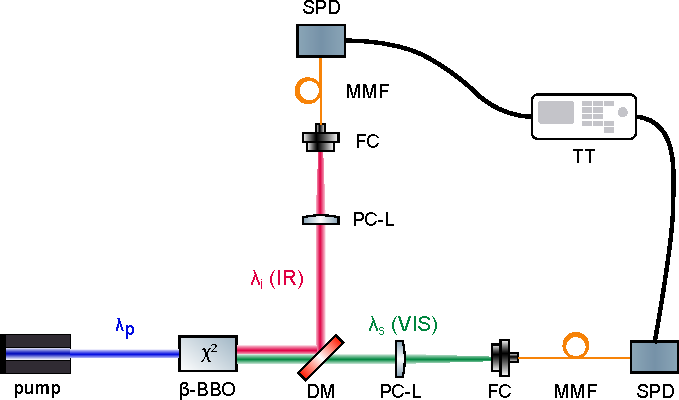
\includegraphics[width=.8\linewidth]{Images/DupishSetupNew.pdf}
    \caption[Experimental setup]{Experimental setup: DM: dichroic mirror, FC: fiber coupling, MMF: multi-mode fiber, PC-L: plano-convex lens, Sam: sample, SPD: single photon detector, TT: time tagging unit}
    \label{fig:setup}
\end{figure}
\todo[inline]{Where is the pump going?}

